\documentclass{acmart}
\usepackage[utf8]{inputenc}
\usepackage{subfig}
\usepackage{graphicx}
\usepackage{sidebyside}
\usepackage{cleveref}
\usepackage{placeins}
\usepackage{colortbl}
\usepackage{bm}

\title{An inquiry into the influence of parallelism and the choice of random
engines on the runtime and results of Stride}

\author{Niels Aerens}
\author{Thomas Avé}
\author{Tobia De Koninck}
\author{Robin Jadoul}

% \date{March 2018}

\begin{abstract}
    In this article, we investigate a few properties of the Stride project. In particular, we look at the influence of the amount of parallelization with respect to the running time of a simulation and the difference in simulation outcomes when varying the used random number generator.
\end{abstract}

\begin{document}

\maketitle

\section{Introduction}
Stride \cite{KUYLEN20172438} is an individual-based Simulator for the Transmission of Infectious Diseases with focus on model flexibility and
performance. The performance of such a simulator is important for the researcher to have fast feedback in order to
build a reasonable model of the disease. The Stride program currently has scenario tests to prevent regressions in the
simulation output. To provide fast feedback to the developers working on Stride the test should run sufficiently quickly.
The running time of the tests are a good indication of the running time of the simulator itself. Hence we perform a
performance analysis of the running time of tests and the influence of parallelism.

The scenario tests are using the Attack Rate as parameter to assert the simulator outcome. Since Stride is a stochastic
system and thus relies on randomness, the output of its tests are variable. Therefore the tests use an acceptability range
for the test outcome. We determined these ranges by running the tested simulations multiple times (100+). We noticed
by using a QQ-Plot and hypothesis tests that the Attack Rate can be considered to follow a normal distribution.
For the accepted ranges, we decided to allow a distance of 2 standard deviations from the observed mean.

The second topic of this paper is to analyze the influence of the random number generator engine on the Attack Rate.
Stride uses the Trng library \cite{bauke2015tina} as random number generator. The inspected engines are \texttt{lgc64}, \texttt{lgc64\_shift}, \texttt{mrg2}, \texttt{mrg3}, \texttt{yarn2} and \texttt{yarn3}.

\pagebreak

\section{Methods}

\subsection{Influence of multi-threading}

The analysis described in this section was performed on a 32 core AMD machine. Therefore the tests were executed with a maximum of 32 threads, which is a reasonable maximum for any workstation at the time of writing. By using a Bash-script\footnote{\url{https://ledfan.github.io/Bachelorproef/assets/src/week4/bench.sh}} % TODO update links to website
the Stride tests were run with an increasing amount of threads, starting at 1 up to 32.

\subsection{Influence of random engine}

Using a Python3 script\footnote{\url{https://ledfan.github.io/Bachelorproef/assets/src/week4/random\_engines.py}} 
the simulation was run using the different random engines, at the same time measuring the running time.

\section{Results}

\subsection{Influence of multi-threading}
The running time in function of the number of threads are shown in \cref{fig:threads}. The difference between the first and third
quartile is only 0.45 seconds. This difference is negligible compared to the 27 seconds running time. Even the furthest outliers are less than 2 seconds apart. We can safely conclude
that the parallelisation of the code doesn’t have a great influence on the performance. There should hopefully be some room for improvement here for the performance of Stride.
Note that for each number of threads, the values are obtained by running the Influenza A simulation 15 times and taking the average running time.

\sidebyside[!hbt][fig:threads:scatter][fig:threads:boxplot]
    {Connected scatter plot}
    {images/performance_scatter.png}
    {Boxplot}
    {images/boxplot_performance.png}
    {Running time in function of number of threads}
    {fig:threads}
\subsection{Influence of random engine}
The engine which needs the least amount of time is the \texttt{lgc64} engine, the \texttt{yarn3} engine requires the most amount of time. The difference in time is 60 seconds when running the tests 15 times, which means that for one run the difference is only about 4 seconds. Thus there isn’t a big difference. A complete comparison of running times can be found in \cref{fig:engine:running}.
The distribution analysis of the results with different random engines was done with 100 data points for each random engine. While this is still a relatively small sample size, much larger sample sizes were not feasible due to the time requirements to run them all.


\begin{figure}
    \centering
    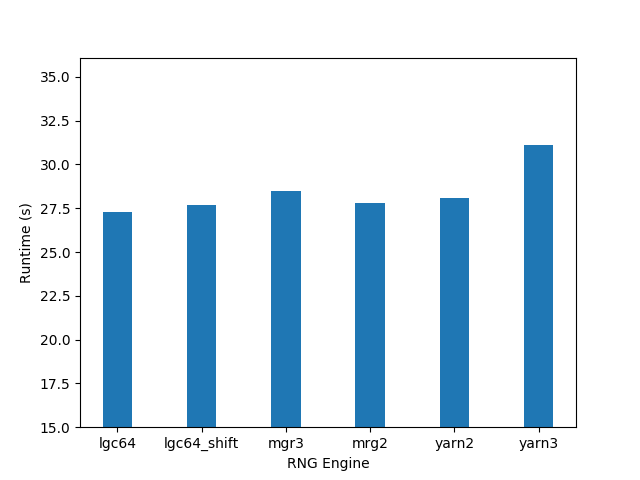
\includegraphics[width=0.7\textwidth]{images/engine_performance_bar.png}
    \caption{Running time of the different rng engines for the influenza A test case.}
    \label{fig:engine:running}
\end{figure}


The first test case of Stride (Influenza A\footnote{\url{https://github.com/LEDfan/Bachelorproef/blob/dd1ef48867238d62446813f47d6718908505b7f2/test/cpp/gtester/BatchRuns.cpp\#L82}})
performs a simulation of influenza in Flanders, with an $R_0$ value\footnote{Basic reproduction number, a measure for the infectiousness of a disease: the amount of people will 1 infected person infect directly in a completely
susceptible population.} of 3.0. For this test case the range of allowed attack rates doesn't change much. 
The second test case (Influenza B\footnote{\url{https://github.com/LEDfan/Bachelorproef/blob/dd1ef48867238d62446813f47d6718908505b7f2/test/cpp/gtester/BatchRuns.cpp\#L86}}) uses a seeding rate of 0, which results in a constant attack rate of 0. As expected the RNG engine doesn't have influence on this outcome.
The same holds for the third test case (Influenza C\footnote{\url{https://github.com/LEDfan/Bachelorproef/blob/dd1ef48867238d62446813f47d6718908505b7f2/test/cpp/gtester/BatchRuns.cpp\#L91}}) which uses a very low seeding rate and a large immunity factor. The attack vector for every engine is 5.
The Measles 16\footnote{\url{https://github.com/LEDfan/Bachelorproef/blob/dd1ef48867238d62446813f47d6718908505b7f2/test/cpp/gtester/BatchRuns.cpp\#L97}} testcase is more interesting for the analysis of the RNG engines. The disease simulated is not influenza but the measles. The $R_0$ value is set to 16, which results in a very large part of the population becoming infected.
The last testcase (Measles 60) sets the $R_0$ value to 60. It infects the whole population, so the attack rate is for all the engines the same.
    
\subsection{Normality of the output}
\label{par:normality}
To validate our assumption that the distribution of the attack rate was normal for our tests, we both looked at QQ-plots and histograms of the outputs of different runs against a reference normal distribution with $\mu = \bar{X}, \sigma=S_X$, verified that histograms had a more or less normal look to them, and verified with the Shapiro-Wilkes test.

% Influenza A
Looking at the Influenza A testcase, we find the resulting P-values for Shapiro-Wilkes test in \cref{tab:influenza_a:shapiro}. Here, all random engines result in an (at least approximately) normal distribution for the attack rate.
\begin{table}[!hbt]
    \begin{tabular}{c c c c c c}
       \textbf{lgc64} & \textbf{lgc64\_shift} & \textbf{mrg2} & \textbf{mrg3} & \textbf{yarn2} & \textbf{yarn3}\\
        0.8719 & 0.4609 & 0.9385 & 0.6556 & 0.7254 & 0.7089
    \end{tabular}
    \caption{P-values of the Influenza A test case for the Shapiro-Wilkes normality test}
    \label{tab:influenza_a:shapiro}
\end{table}


% Measles 16
For the Measles 16 testcase, resulting P-values for the Shapiro-Wilkes test can be found in \cref{tab:measles_16:shapiro}.

\begin{table}[!hbt]
    \begin{tabular}{c c c c c c}
       \textbf{lgc64} & \textbf{lgc64\_shift} & \textbf{mrg2} & \textbf{mrg3} & \textbf{yarn2} & \textbf{yarn3}\\
        0.8231 & 0.4216 & 0.9115 & 0.4199 & 0.1473 & 0.4431
    \end{tabular}
    \caption{P-values of the Measles 16 test case for the Shapiro-Wilkes normality test}
    \label{tab:measles_16:shapiro}
\end{table}

We can consider the attack rate to be normally distributed in all presented cases.

A few of the plots can be seen in \cref{fig:normality}, and for those who would like to see more of them, they can be generated with the script and datafiles found at our website\footnote{\url{https://ledfan.github.io/Bachelorproef/assets/src/week4/random\_engines\_stats.py}}.

\begin{figure}%
   	\makebox[\textwidth][c]{%
   		\centering%
   		\subfloat[QQ plot of Influenza A results with \texttt{lgc64}]{%
   			{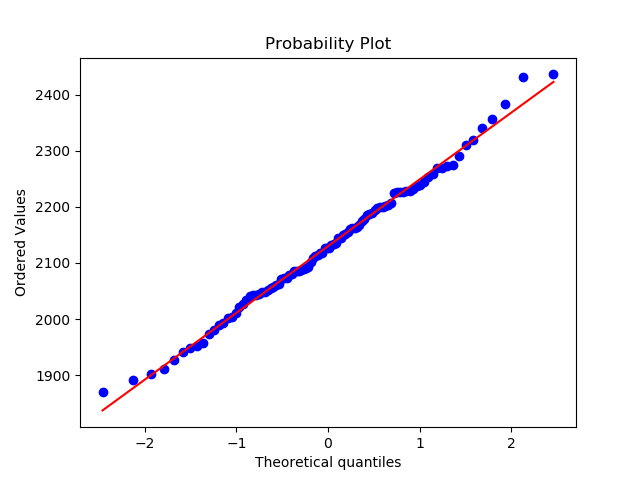
\includegraphics[width=0.5\textwidth]{images/influenza_qq_lgc64.png}}%
   		}%
   		\qquad%
   		\subfloat[Histogram of Influenza A results with \texttt{lgc64}]{%
  			{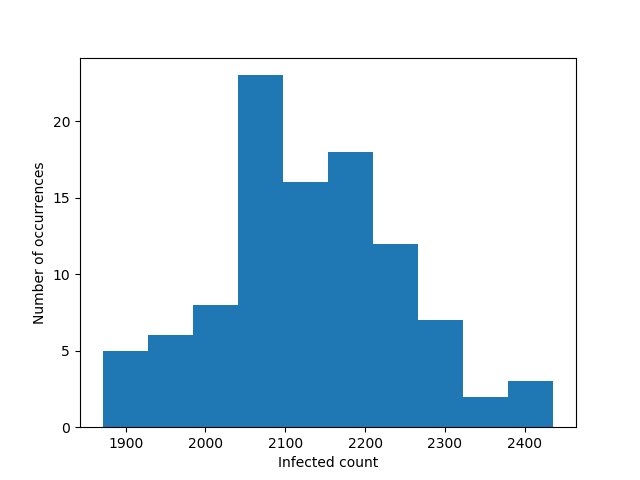
\includegraphics[width=0.5\textwidth]{images/influenza_histo_lgc64.png}}%
   		}%
   	}\\
   	\makebox[\textwidth][c]{%
   		\centering%
   		\subfloat[QQ plot of Measles 16 results with \texttt{mrg2}]{%
   			{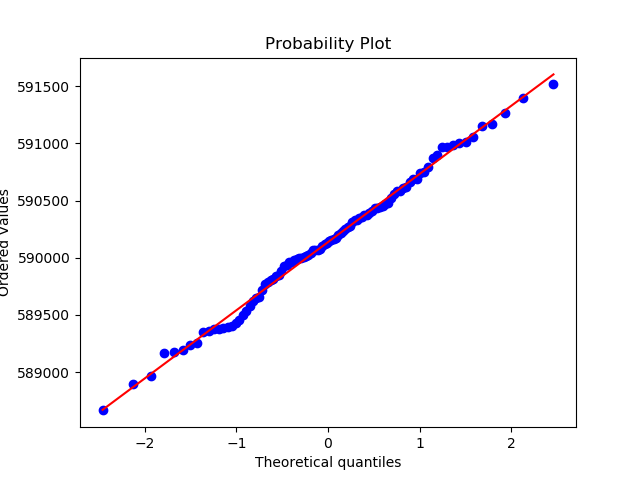
\includegraphics[width=0.5\textwidth]{images/measles_qq_mrg2.png}}%
   		}%
   		\qquad%
   		\subfloat[Histogram of Measles 16 results with \texttt{mrg2}]{%
  			{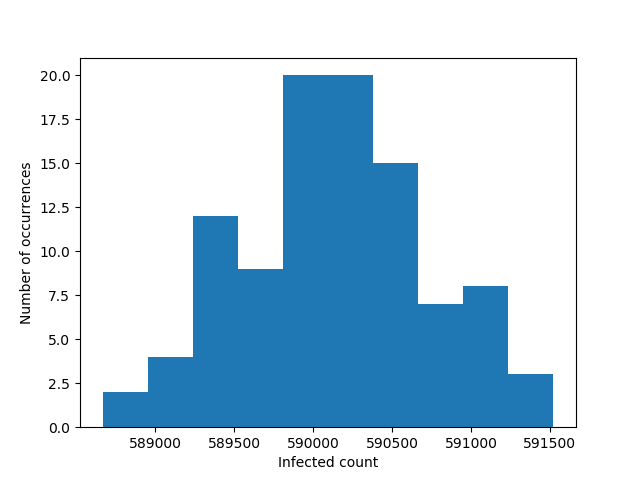
\includegraphics[width=0.5\textwidth]{images/measles_histo_mrg2.png}}%
   		}%
   	}%
   	\label{fig:normality}
   	\caption{Visually evaluating the normality of the attack rate}
\end{figure}

\subsection{Equality of acceptable ranges for the test cases}

In this section the equality of the different value ranges which are accepted by the tests for each random engine is verified. Only the Influenza A and Measles 16 test cases are studied since they provide a variable range. The tests are done using a Levene test for the standard deviations and a t-test for related samples for the means.

The hypotheses for the Levene test:
\[
\begin{aligned}
 H_0 &: \sigma_1 = \sigma_2\\
 H_1 &: \sigma_1 \ne \sigma_2\
\end{aligned}
\]

and for the t-test:
\[
\begin{aligned}
 H_0 &: \mu_1 = \mu_2  \\
 H_1 &: \mu_1 \ne \mu_2.
\end{aligned}
\]

The p-values for these tests are listed in \cref{tab:influenza:p_values} and \cref{tab:measles_16:p_values}. They clearly indicate that the \(H_0\) should not be rejected for both tests on a confidence level of $\alpha = 0.05$. Consequently, we can fairly confidently conclude that the distribution of the attack rate does not differ significantly when using a different random engine.


\begin{table}[!hbt]
    \centering
    \bgroup
    \def\arraystretch{2}
    \begin{tabular}{c|c|c|c|c|c}
                                & \textbf{Influenza A}  & \textbf{Measles 16} \\ \hline
        \texttt{lgc64}          & \([1896, 2364]\)       & \([588959, 591317]\) \\
        \texttt{lgc64\_shift}   & \([1893, 2372]\)       & \([588992, 591360]\) \\
        \texttt{mrg2}           & \([1899, 2334]\)       & \([588967, 591307]\) \\
        \texttt{mrg3}           & \([1891, 2345]\)       & \([589012, 591268]\) \\
        \texttt{yarn2}          & \([1879, 2331]\)       & \([588836, 591615]\) \\
        \texttt{yarn3}          & \([1902, 2331]\)       & \([588751, 591443]\) \\
    \end{tabular}
    \egroup
    \caption{The acceptable attack rates for the Influenza A en Measles 16 test case for every random number engine}
    \label{tab:ranges_engines}
\end{table}

\begin{table}[!hbt]
    \centerline{\begin{tabular}{c|c|c|c|c|c|}
        & \textbf{lgc64} & \textbf{lgc64\_shift} & \textbf{mrg2} & \textbf{mrg3} & \textbf{yarn2} \\
        &  \( \bm{p_\mu} \quad \bm{p_\sigma} \)
            &  \( \bm{p_\mu} \quad \bm{p_\sigma} \)
            &  \( \bm{p_\mu} \quad \bm{p_\sigma} \)
            &  \( \bm{p_\mu} \quad \bm{p_\sigma} \)
            &  \( \bm{p_\mu} \quad \bm{p_\sigma} \) \\
        \textbf{lgc64\_shift}
            & \( 0.8819 \quad 0.7593 \)
            & \cellcolor{gray}
            & \cellcolor{gray}
            & \cellcolor{gray}
            & \cellcolor{gray} \\
        \textbf{mrg2}      
            & \( 0.2797 \quad 0.3763 \) 
            & \( 0.3359 \quad 0.2392 \) 
            & \cellcolor{gray}
            & \cellcolor{gray}
            & \cellcolor{gray} \\
        \textbf{mrg3}          
            & \( 0.3942 \quad 0.7113 \)
            & \( 0.3958 \quad 0.5026 \) 
            & \( 0.8842 \quad 0.6079 \) 
            & \cellcolor{gray}
            & \cellcolor{gray} \\
        \textbf{yarn2}        
            & \( 0.1507 \quad  0.5990 \)  
            & \( 0.1432 \quad 0.4116 \)  
            & \( 0.4590 \quad 0.7271 \) 
            & \( 0.4339 \quad 0.8737 \)  
            & \cellcolor{gray} \\
        \textbf{yarn3}          
            & \( 0.3578 \quad 0.4295 \)  
            & \( 0.3351 \quad 0.2750  \) 
            & \( 0.9843 \quad 0.9042  \)
            & \( 0.9017 \quad 0.6833 \) 
            & \( 0.4517 \quad 0.8102  \) \\
    \end{tabular}}
    \caption{P-values of the Influenza A test case}
    \label{tab:influenza:p_values}
\end{table}

\begin{table}[!hbt]
    \begin{tabular}{c|c|c|c|c|c|c}
        & \textbf{lgc64} & \textbf{lgc64\_shift} & \textbf{mrg2} & \textbf{mrg3} & \textbf{yarn2} \\
        &  \( \bm{p_\mu} \quad \bm{p_\sigma} \)
            &  \( \bm{p_\mu} \quad \bm{p_\sigma} \)
            &  \( \bm{p_\mu} \quad \bm{p_\sigma} \)
            &  \( \bm{p_\mu} \quad \bm{p_\sigma} \)
            &  \( \bm{p_\mu} \quad \bm{p_\sigma} \) \\
        \textbf{lgc64\_shift}
            & \( 0.2164 \quad 0.8855 \)
            & \cellcolor{gray}
            & \cellcolor{gray}
            & \cellcolor{gray}
            & \cellcolor{gray} \\
        \textbf{mrg2}      
            & \( 0.9754 \quad 0.8673 \) 
            & \( 0.2264 \quad 0.9838 \) 
            & \cellcolor{gray}
            & \cellcolor{gray}
            & \cellcolor{gray} \\
        \textbf{mrg3}          
            & \( 0.9630 \quad 0.9900 \)
            & \( 0.2671 \quad 0.8882 \) 
            & \( 0.9373 \quad 0.8687 \) 
            & \cellcolor{gray}
            & \cellcolor{gray} \\
        \textbf{yarn2}        
            & \( 0.3326 \quad 0.2670 \)  
            & \( 0.5949 \quad 0.2232 \)  
            & \( 0.3163 \quad 0.2107 \) 
            & \( 0.3081 \quad 0.2400 \)  
            & \cellcolor{gray} \\
        \textbf{yarn3}          
            & \( 0.6517 \quad 0.5366 \)  
            & \( 0.3611 \quad 0.4624 \) 
            & \( 0.6508 \quad 0.4457 \)
            & \( 0.6282 \quad 0.5097 \) 
            & \( 0.2195 \quad 0.6542 \) \\
    \end{tabular}
    \caption{P-values of the Measles 16 test case}
    \label{tab:measles_16:p_values}
\end{table}

\section{Future work}

With respect to the analysis performed in this paper, it would be interesting to see an investigation of the influence of threading on the attack rate, or another representative metric of the output of the Stride simulator. It is clear that we hope and expect this effect to be minimal to nonexistent, but it is a good sanity check of the Stride codebase that this would be verified.

\section{Postscriptum}

This analysis was done using commit \texttt{5563ebd337ae75ed35b739307afe03bdb5219325} of the \href{https://github.com/LEDfan/Bachelorproef}{LEDfan/Bachelorproef} repository, corresponding to the \texttt{fde6c507e8596bde6d632f6759c9e65f4b878a68} commit in the upstream \href{https://github.com/broeckho/stride}{broeckho/stride} repository.

\clearpage

\bibliographystyle{ACM-Reference-Format}
\bibliography{references.bib}

\end{document}
